\chapter*{Le Kerala de Munnar à Kovalam\markboth{Le Kerala de Munnar à Kovalam}{}}
\section*{15 novembre 2015}
Longue descente et quelques cols pour revenir sur la côte, il m'arrive de faire quelques dizaines de km sans croiser personne, c'est rare en Inde ! 
\begin{center} 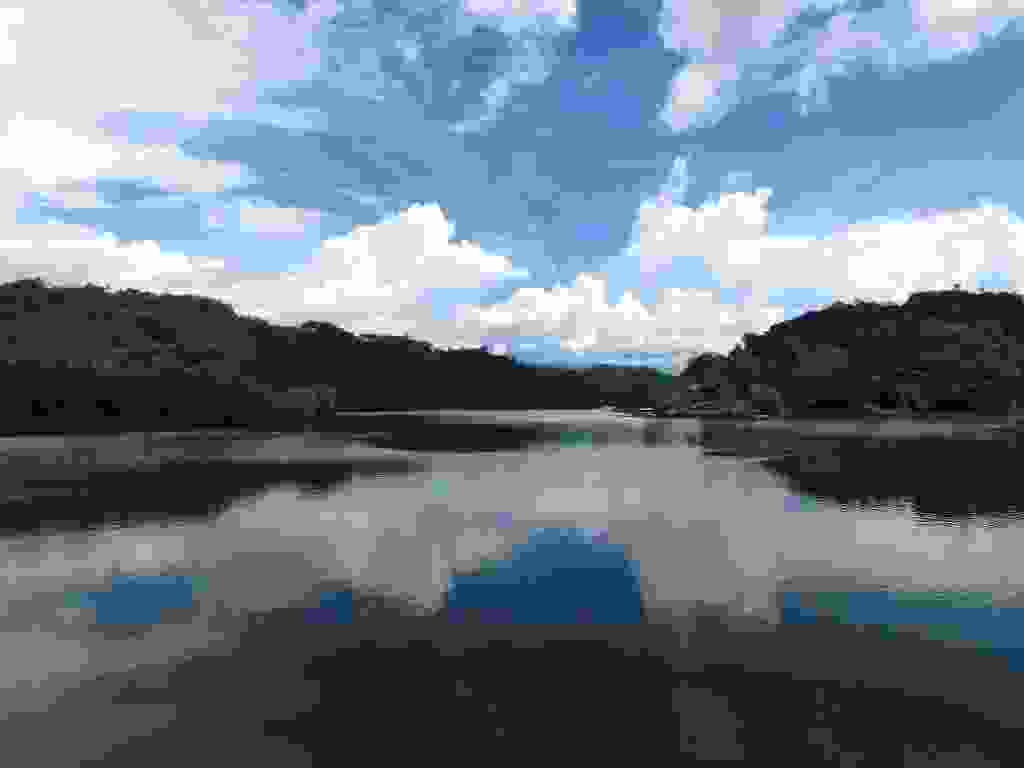
\includegraphics[width=\mywidth]{../wp-content/uploads/2015/11/wpid-oi0001863-1024x768.jpg} \end{center}
\begin{center} 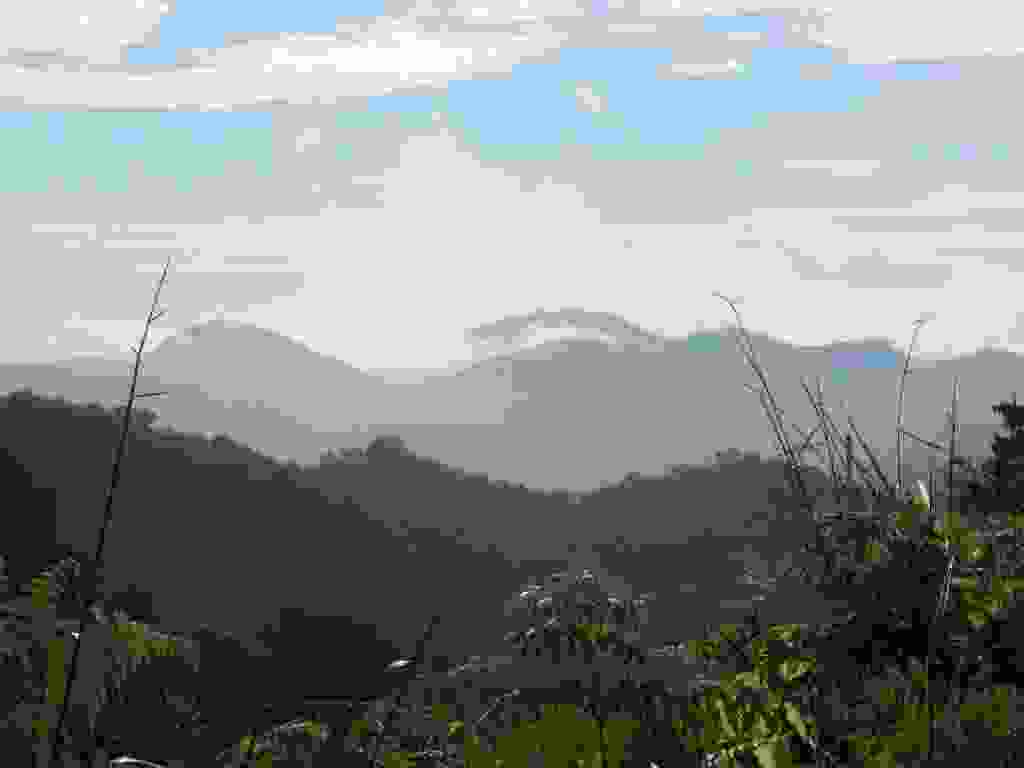
\includegraphics[width=\mywidth]{../wp-content/uploads/2015/11/wpid-oi0002643-1024x768.jpg} \end{center}
\begin{center} 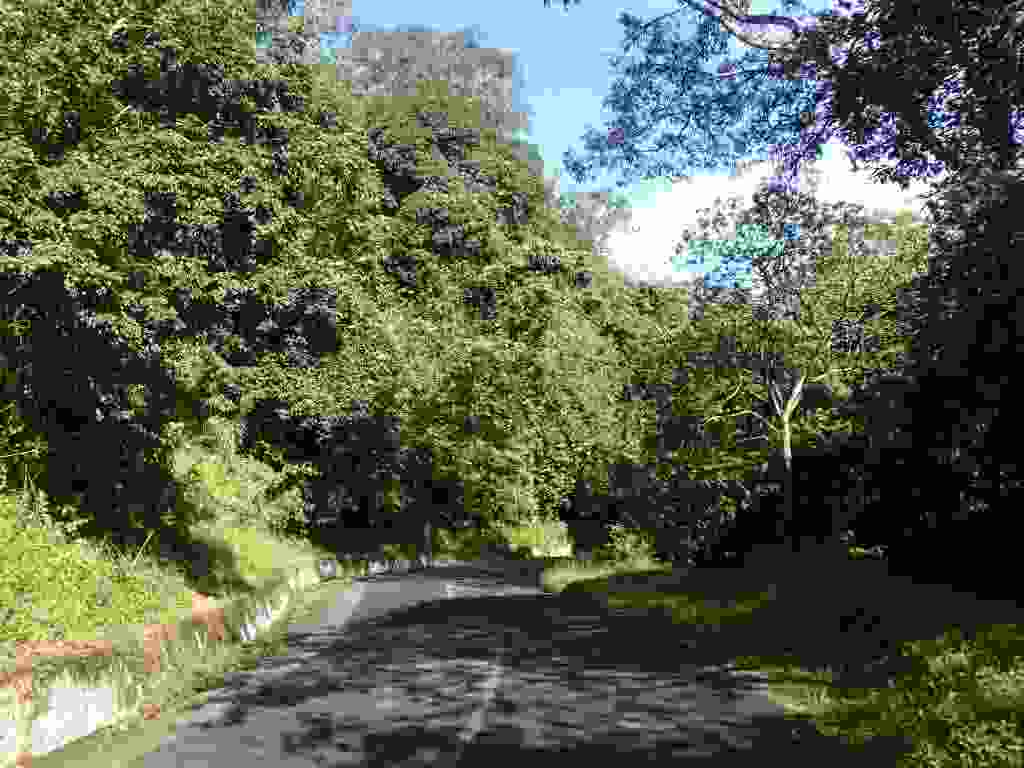
\includegraphics[width=\mywidth]{../wp-content/uploads/2015/11/wpid-oi0002653-1024x768.jpg} \end{center}
\begin{center} 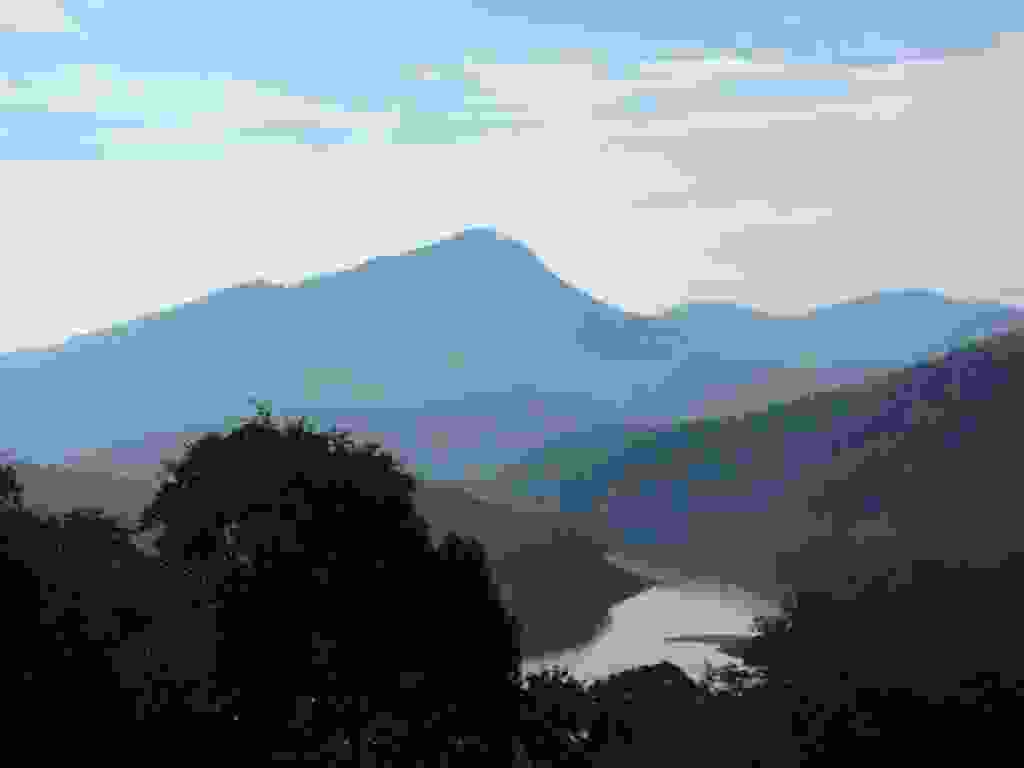
\includegraphics[width=\mywidth]{../wp-content/uploads/2015/11/wpid-oi0002672-1024x768.jpg} \end{center}
\begin{center} 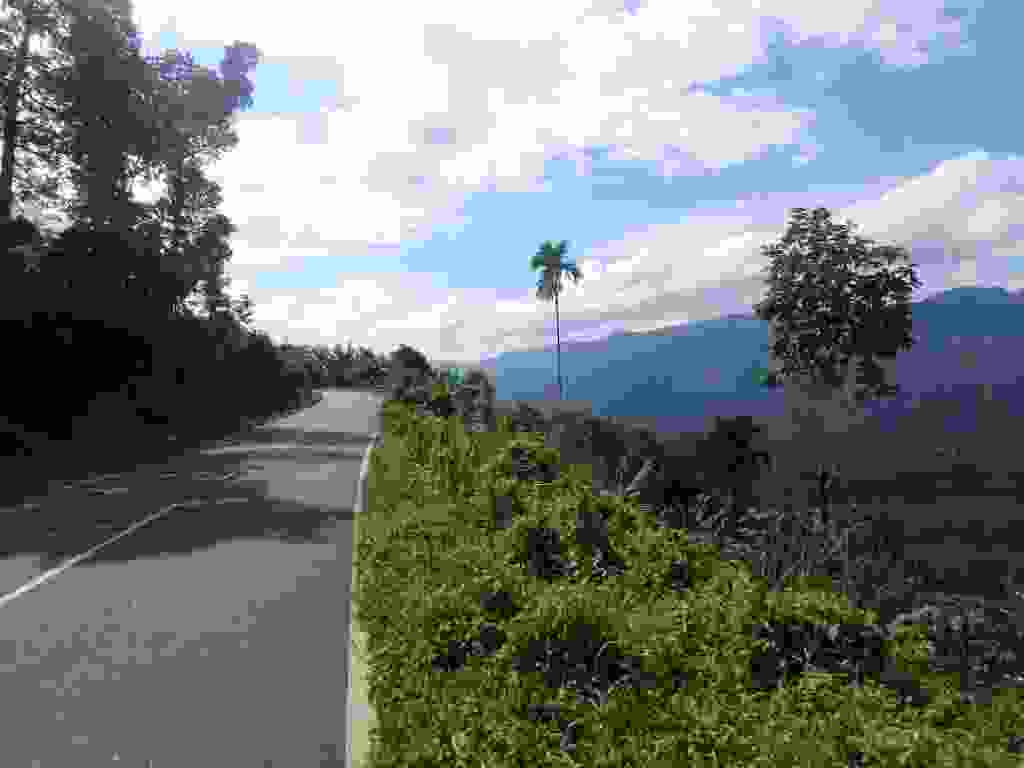
\includegraphics[width=\mywidth]{../wp-content/uploads/2015/11/wpid-oi0002802-1024x768.jpg} \end{center}

\pagebreak
 La seule nuit de camping en Inde pour le moment : le temps de monter la tente j'avais plein de petites sangsues collées aux pieds, sympa ! 
\begin{center} 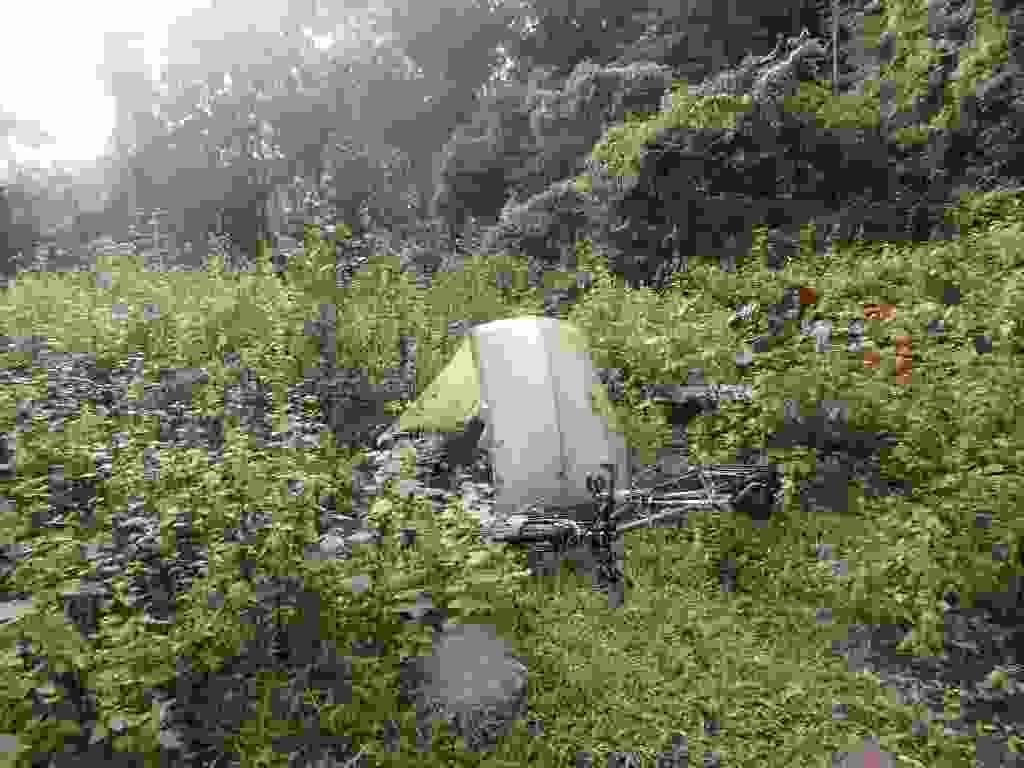
\includegraphics[width=\mywidth]{../wp-content/uploads/2015/11/wpid-oi0002623-1024x768.jpg} \end{center}

 Je repasse là où j'étais hébergé avec le groupe de français, le manager avait contacté un reporter d'un journal local pour faire une interview sur le voyage. Pas évident vu qu'il ne parlait pas anglais...
\begin{center} 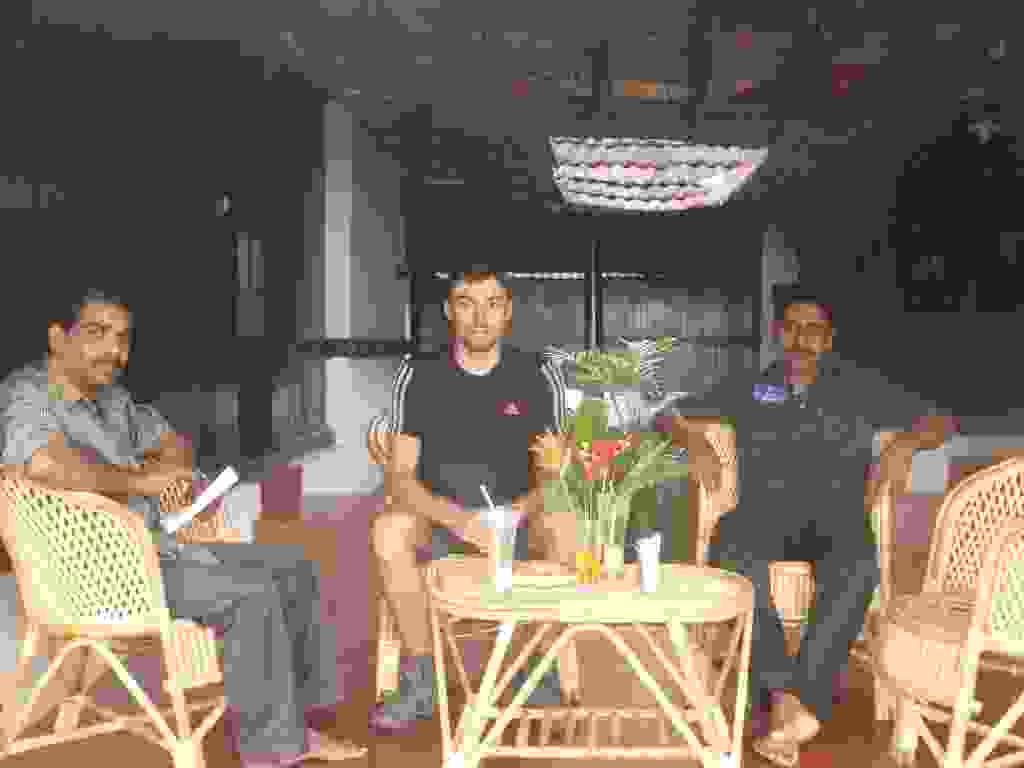
\includegraphics[width=\mywidth]{../wp-content/uploads/2015/11/wpid-oi000315-1024x768.jpg} \end{center}
\begin{center} 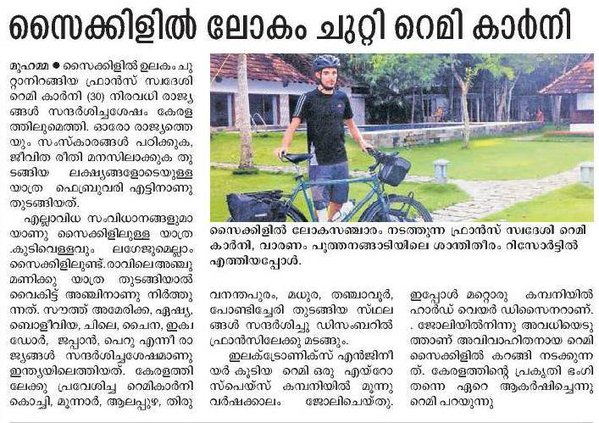
\includegraphics[width=0.65\textwidth]{../wp-content/uploads/2015/11/journal.jpg} \end{center}

 Puis je roule vers le sud et la ville d'Alleppey. 
\begin{center} 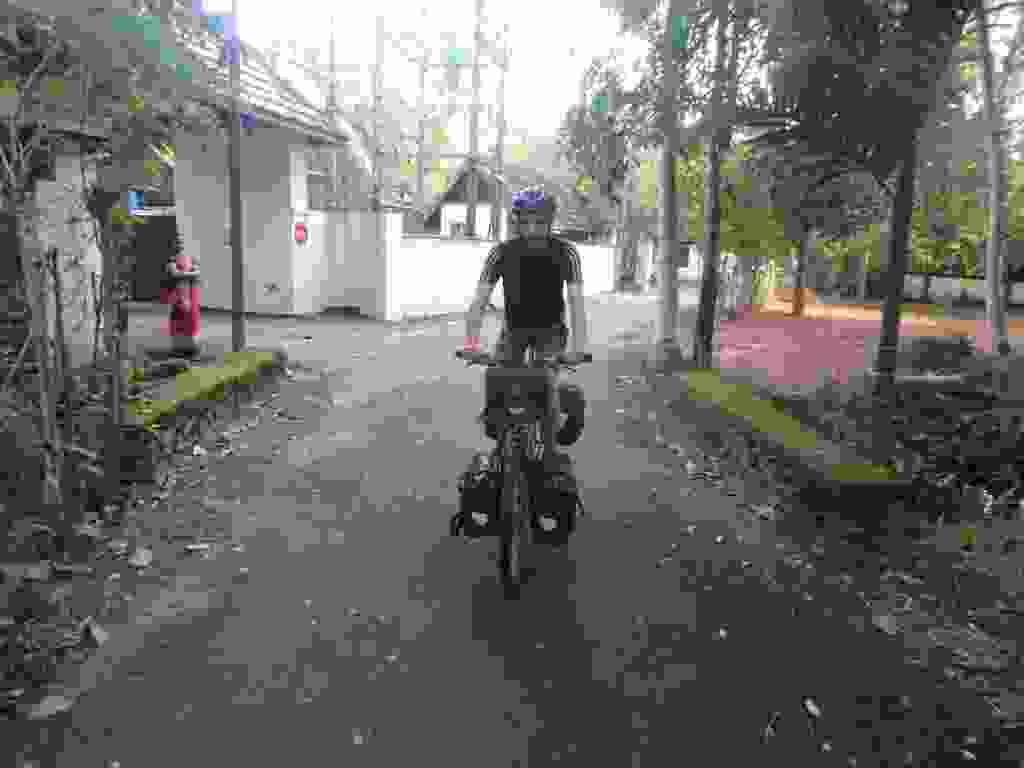
\includegraphics[width=\mywidth]{../wp-content/uploads/2015/11/wpid-oi000321-1024x768.jpg} \end{center}

\pagebreak
 Beau coucher de soleil en arrivant. 
\begin{center} 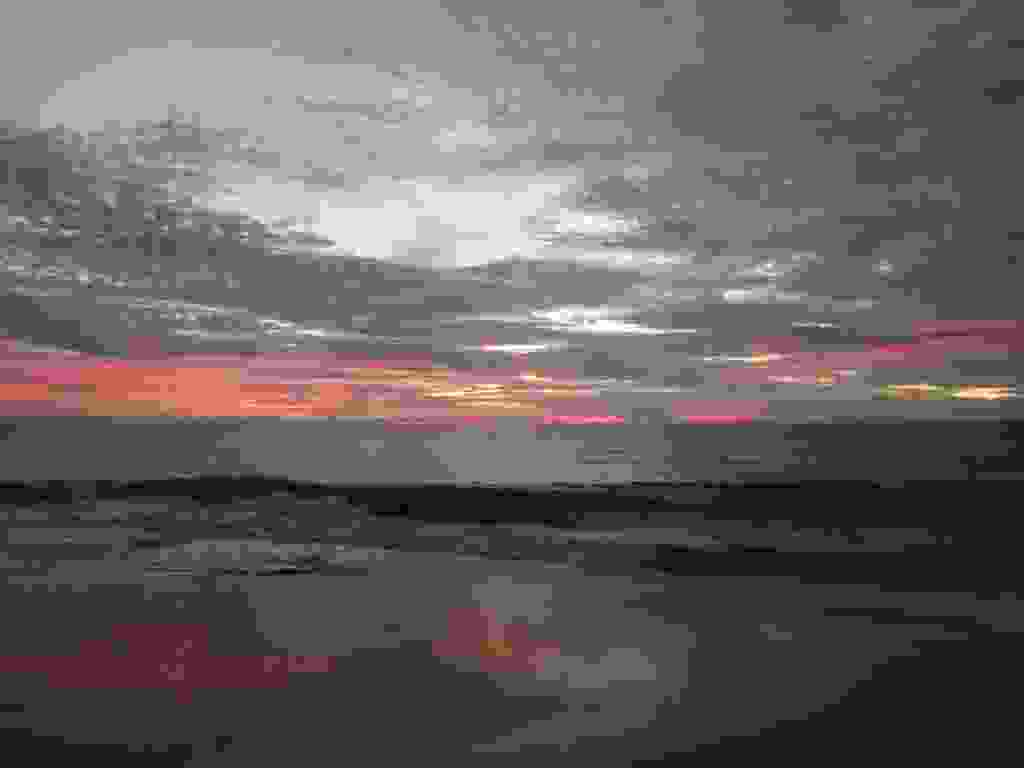
\includegraphics[width=\mywidth]{../wp-content/uploads/2015/11/wpid-oi000324-1024x768.jpg} \end{center}
\begin{center} 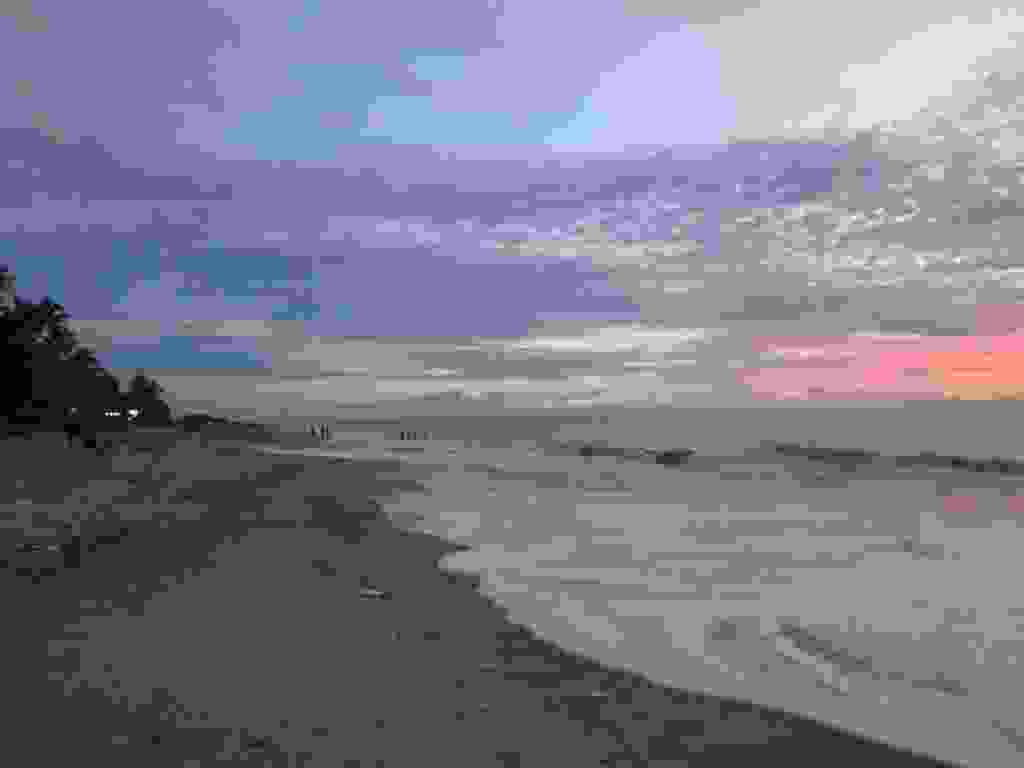
\includegraphics[width=\mywidth]{../wp-content/uploads/2015/11/wpid-oi000326-1024x768.jpg} \end{center}

\pagebreak
  Je prends des petites routes le long de la côte, j'observe le retour des bateaux de pêche sur une plage. 
\begin{center} 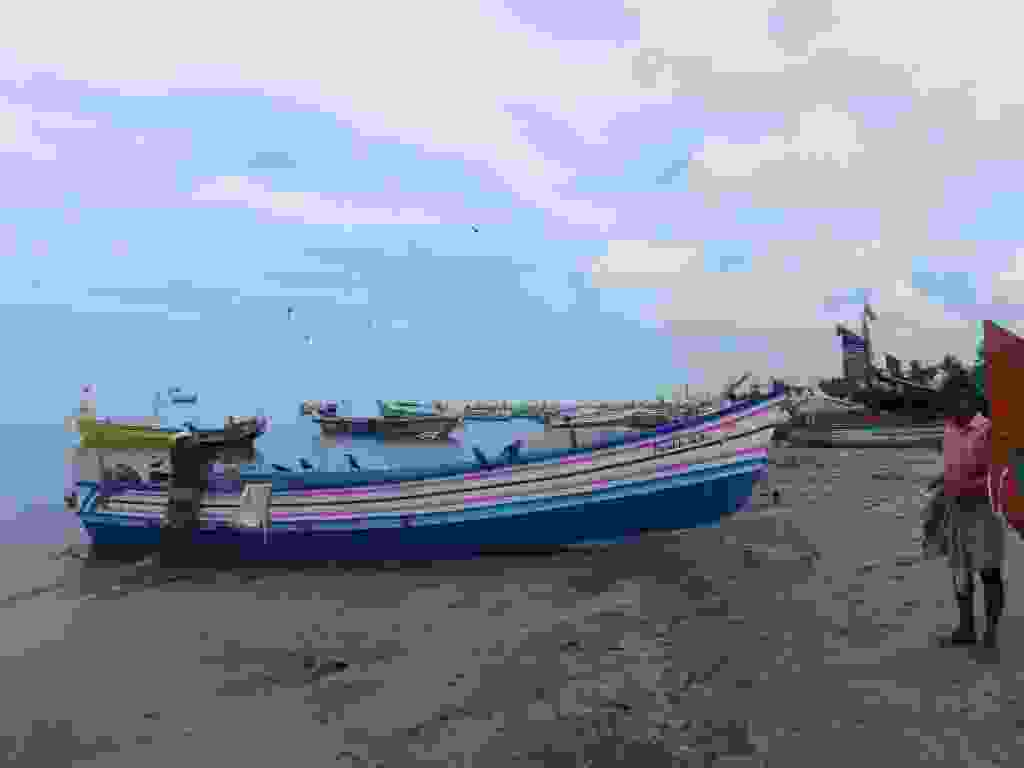
\includegraphics[width=\mywidth]{../wp-content/uploads/2015/11/wpid-oi000334-1024x768.jpg} \end{center}
\begin{center} 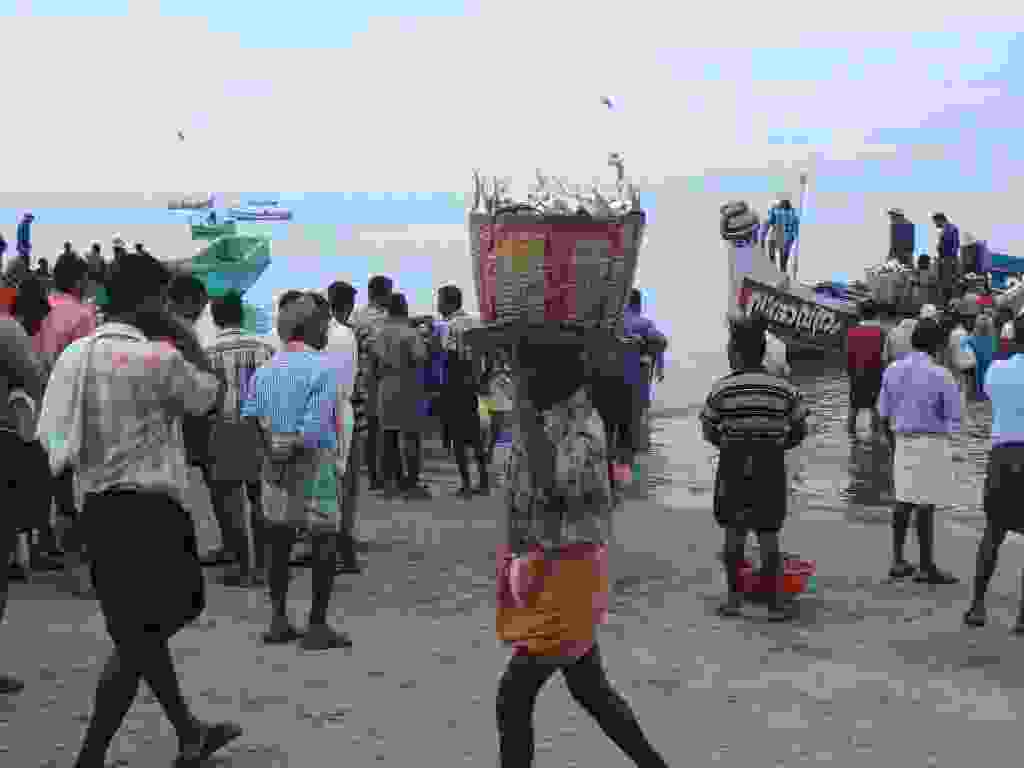
\includegraphics[width=\mywidth]{../wp-content/uploads/2015/11/wpid-oi000333-1024x768.jpg} \end{center}
\begin{center} 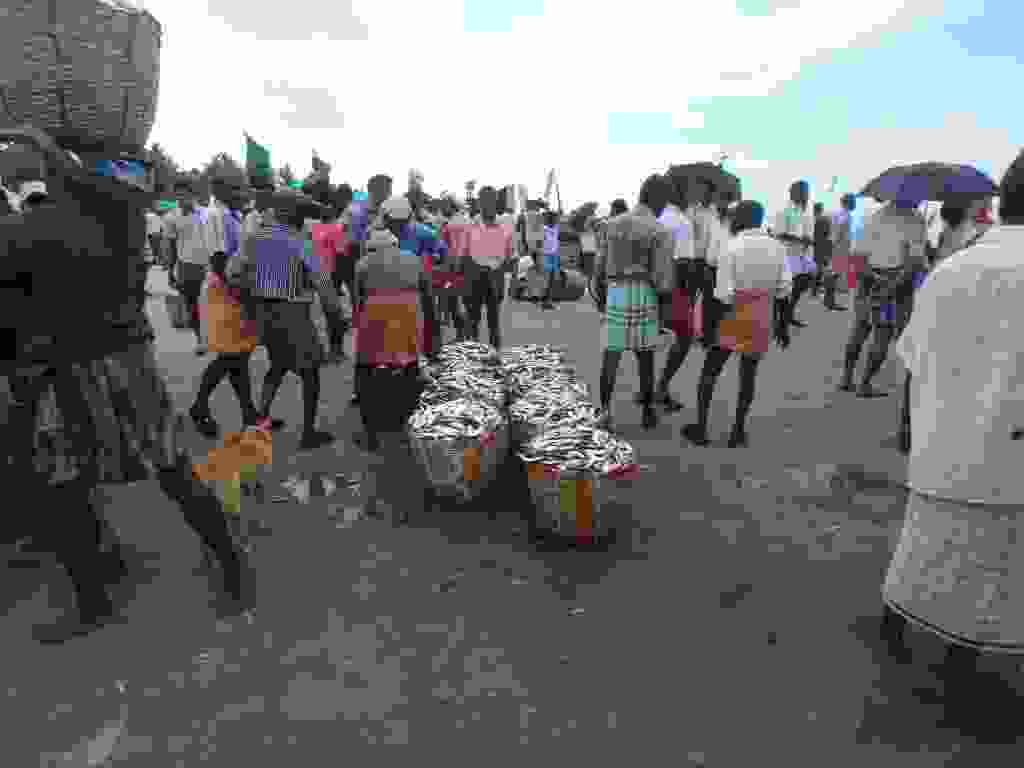
\includegraphics[width=\mywidth]{../wp-content/uploads/2015/11/wpid-oi000336-1024x768.jpg} \end{center}

 Dans un village, des gens en train de jouer aux billes. 
\begin{center} 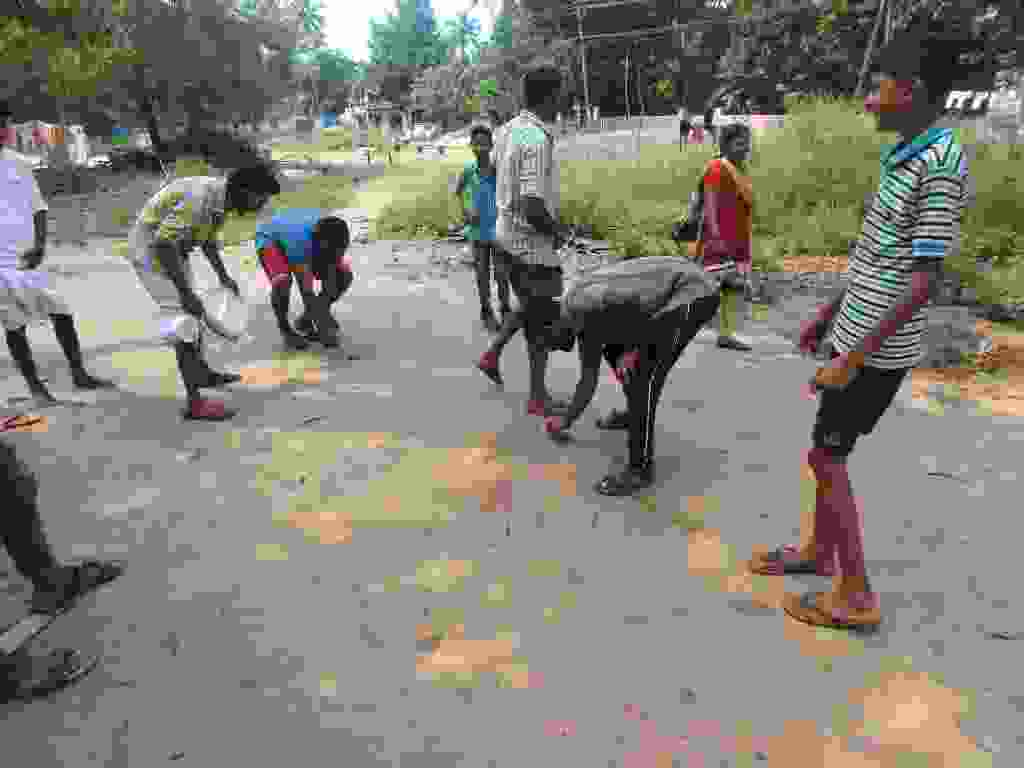
\includegraphics[width=\mywidth]{../wp-content/uploads/2015/11/wpid-oi000338-1024x768.jpg} \end{center}
\begin{center} 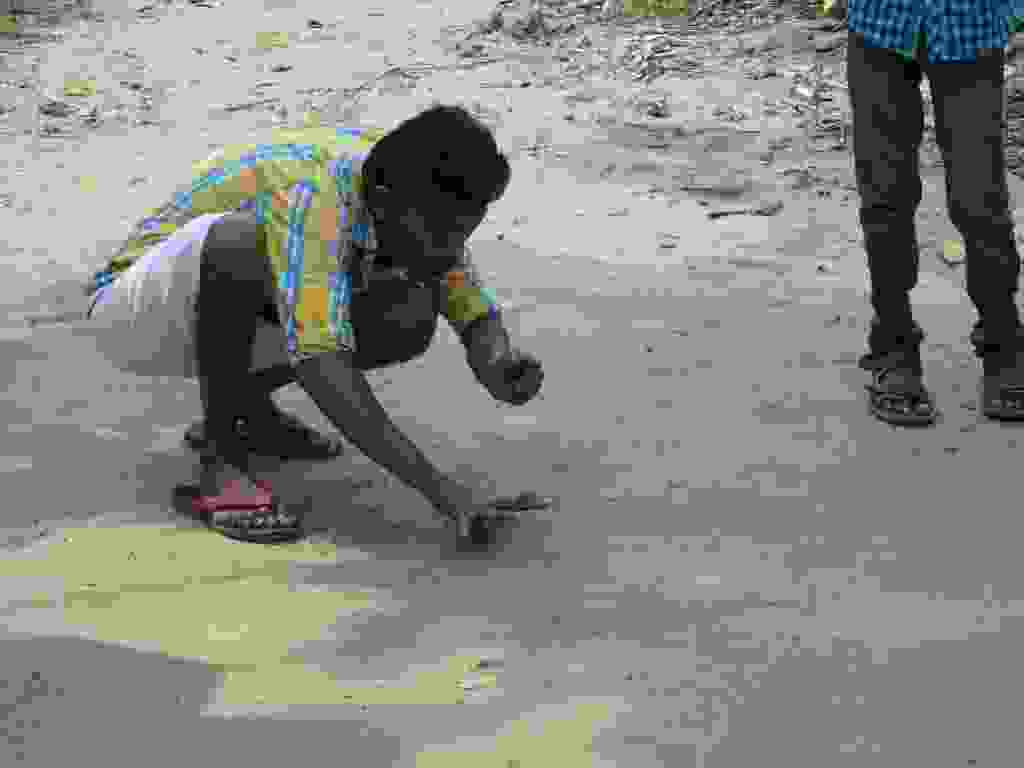
\includegraphics[width=\mywidth]{../wp-content/uploads/2015/11/wpid-oi000339-1024x768.jpg} \end{center}

 Petit détour pour visiter le temple d'Ambalapuzha. 
\begin{center} 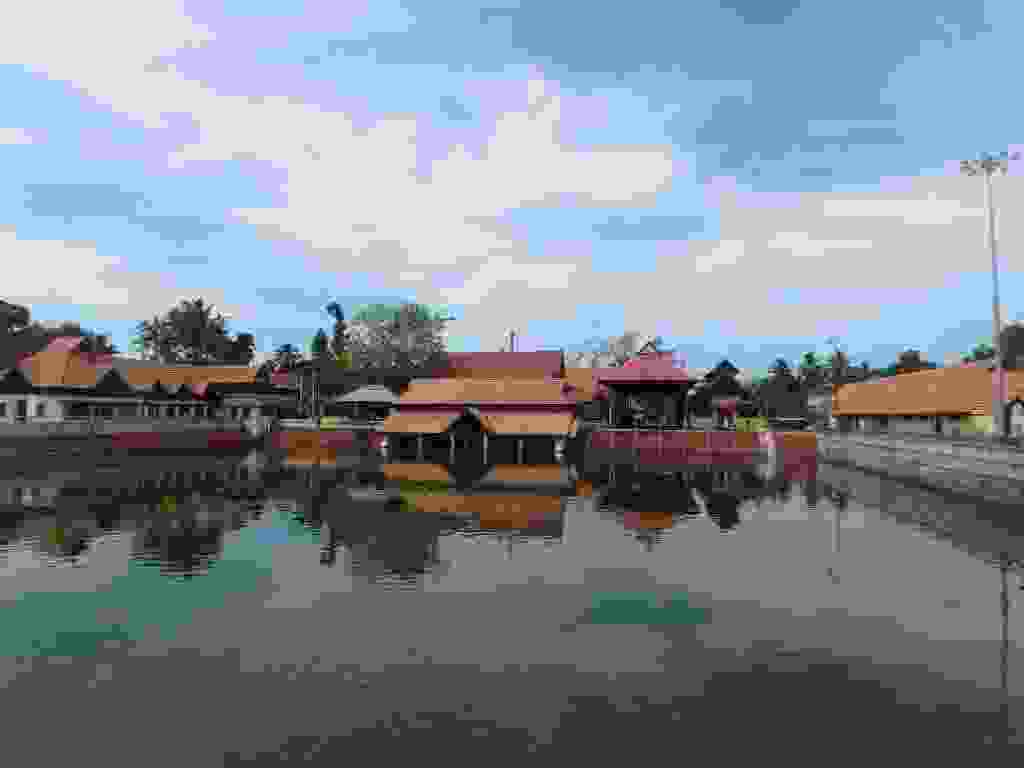
\includegraphics[width=\mywidth]{../wp-content/uploads/2015/11/wpid-oi000346-1024x768.jpg} \end{center}
\begin{center} 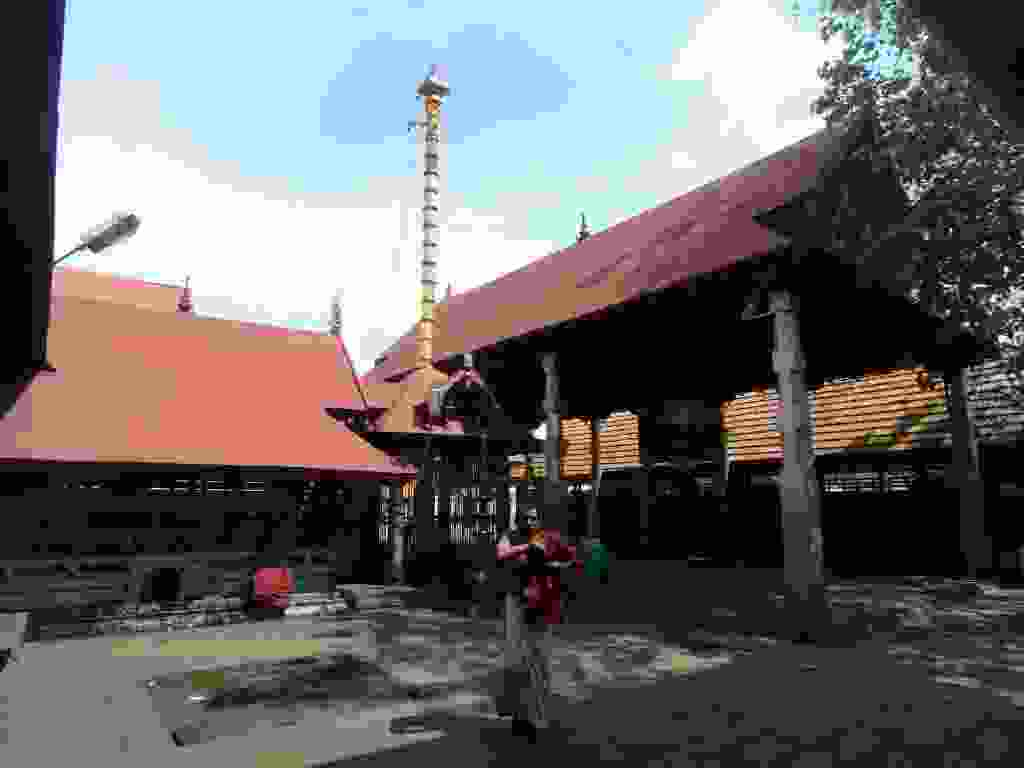
\includegraphics[width=\mywidth]{../wp-content/uploads/2015/11/wpid-oi000342-1024x768.jpg} \end{center}
\begin{center} 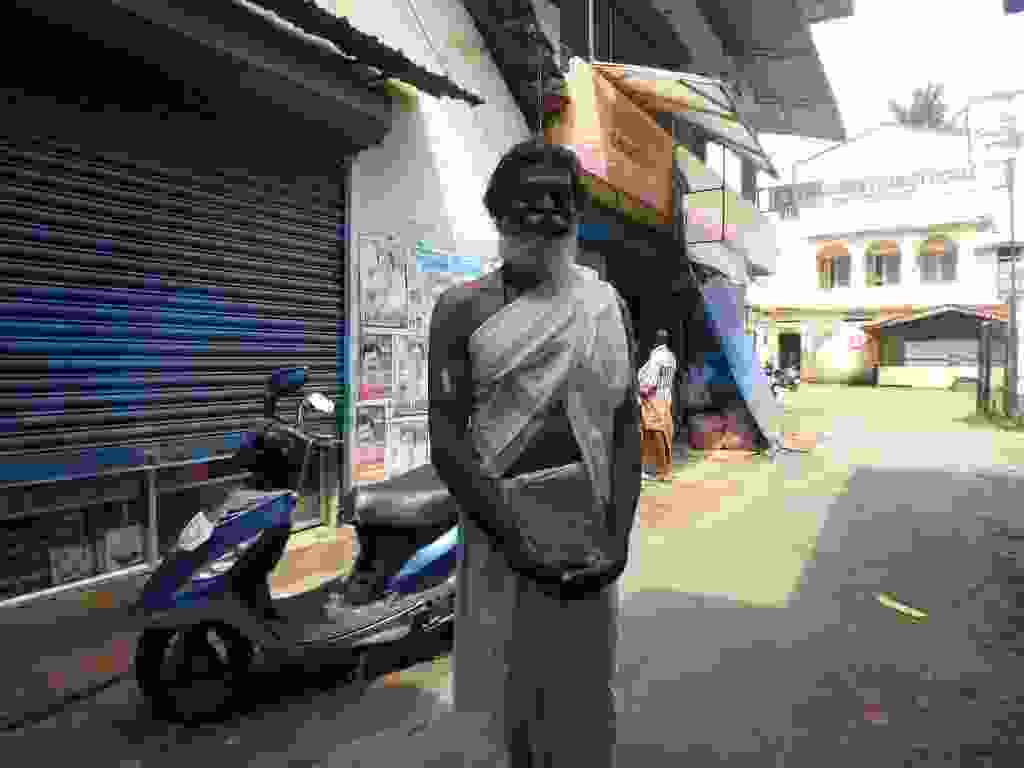
\includegraphics[width=\mywidth]{../wp-content/uploads/2015/11/wpid-oi000347-1024x768.jpg} \end{center}
\begin{center} 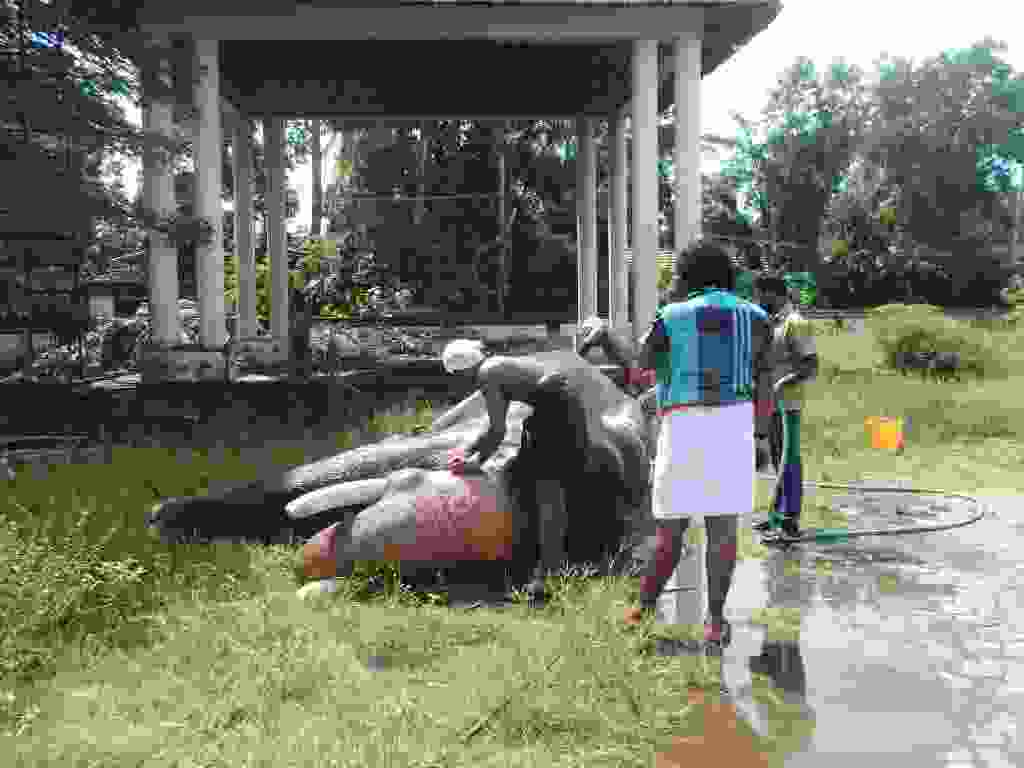
\includegraphics[width=\mywidth]{../wp-content/uploads/2015/11/wpid-oi000344-1024x768.jpg} \end{center}

 Palais de Krishnapuram, belle peinture murale. Également une exposition de sculptures mais pas d'électricité pendant la visite, on ne voyait rien. 
\begin{center} 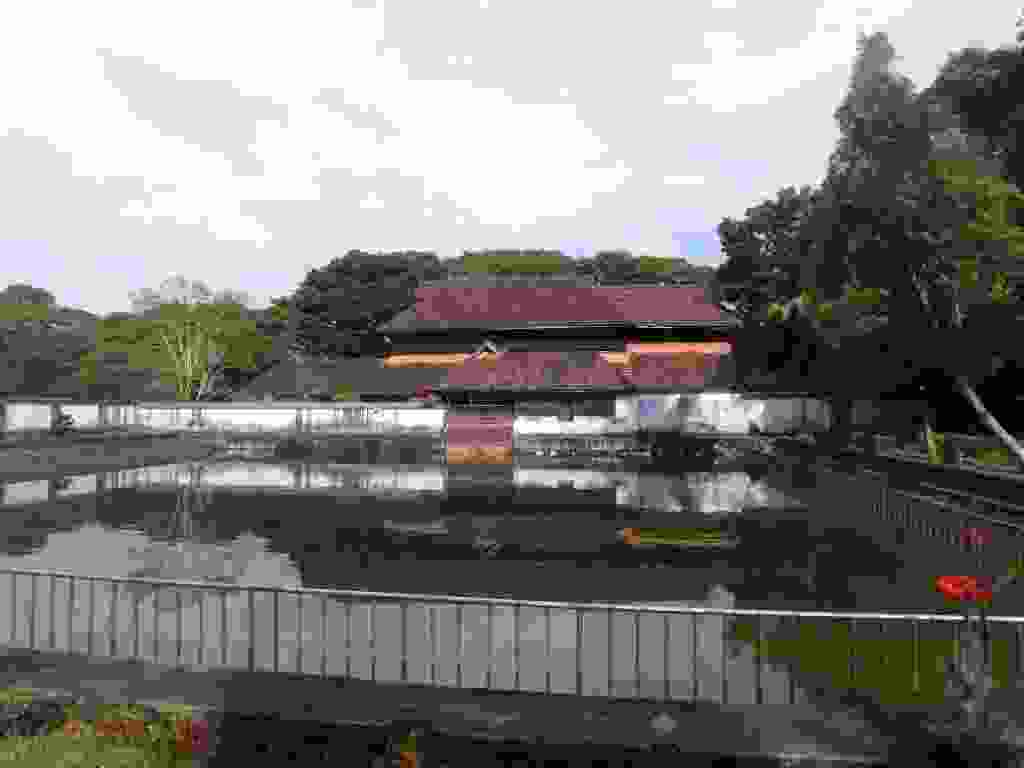
\includegraphics[width=\mywidth]{../wp-content/uploads/2015/11/wpid-oi000359-1024x768.jpg} \end{center}
\begin{center} 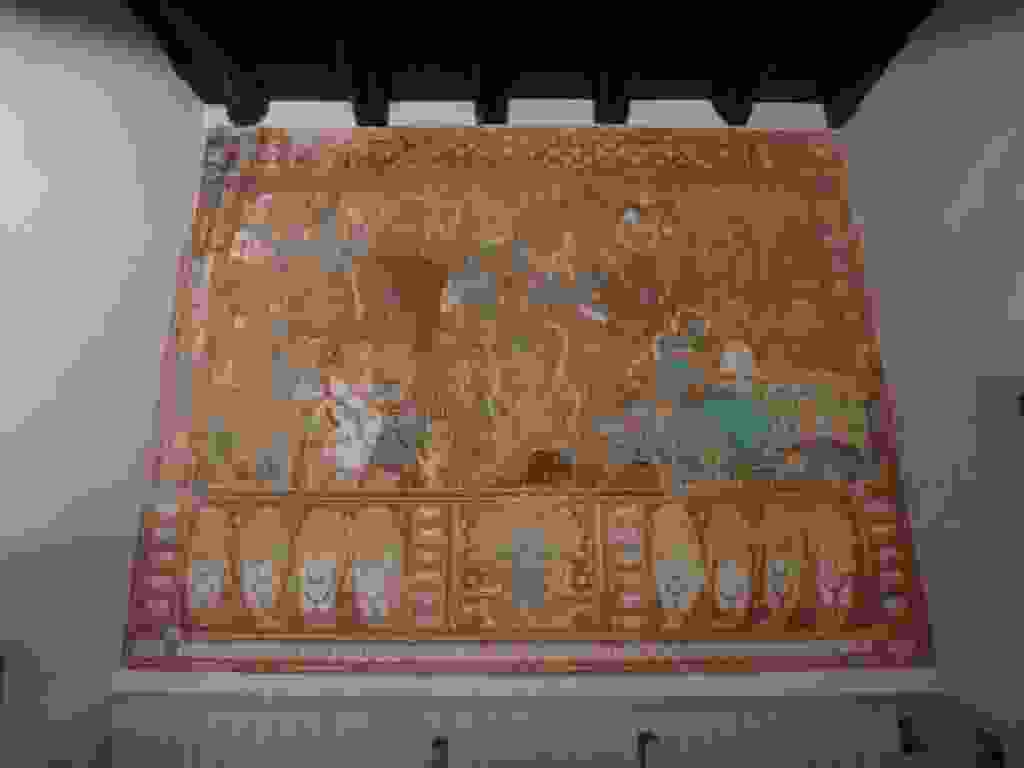
\includegraphics[width=\mywidth]{../wp-content/uploads/2015/11/wpid-oi000351-1024x768.jpg} \end{center}

 J'arrive ensuite à Varkala par un petit chemin au bord de la mer. 
\begin{center} 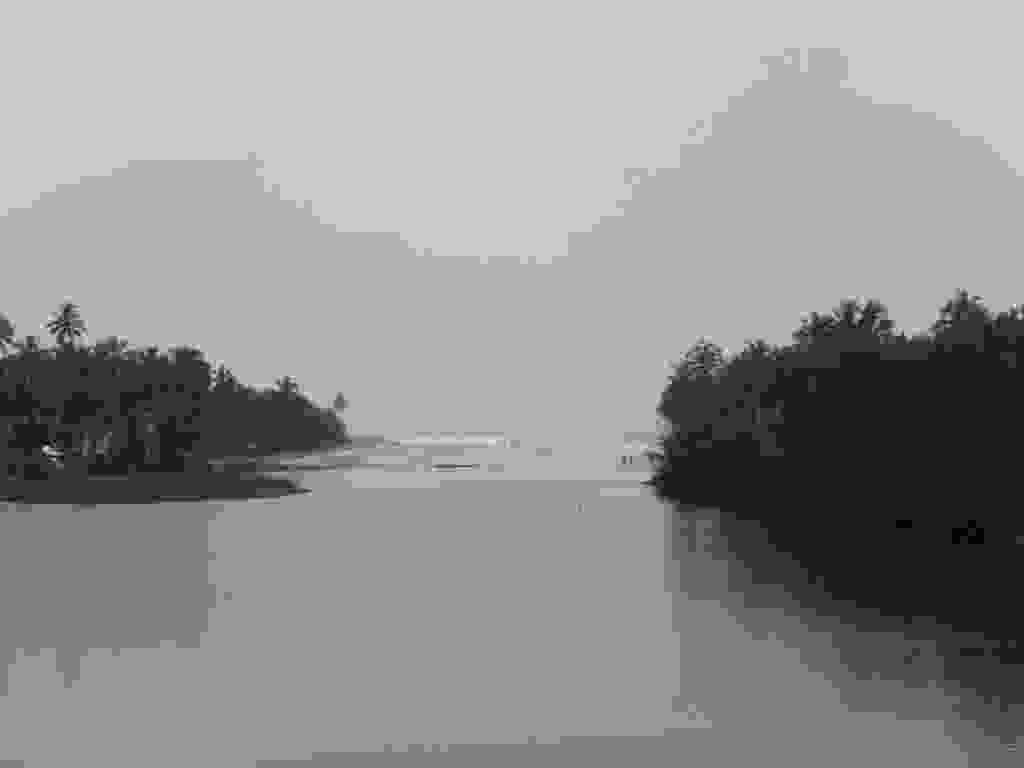
\includegraphics[width=\mywidth]{../wp-content/uploads/2015/11/wpid-oi000368-1024x768.jpg} \end{center}
\begin{center} 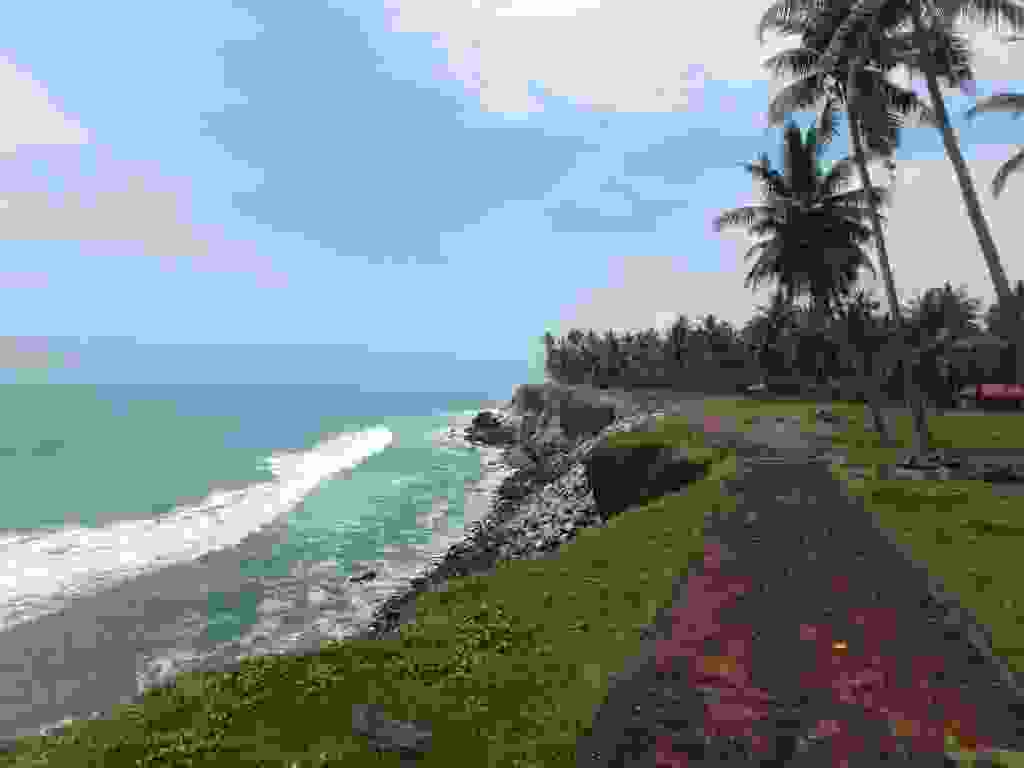
\includegraphics[width=\mywidth]{../wp-content/uploads/2015/11/wpid-oi000370-1024x768.jpg} \end{center}
\begin{center} 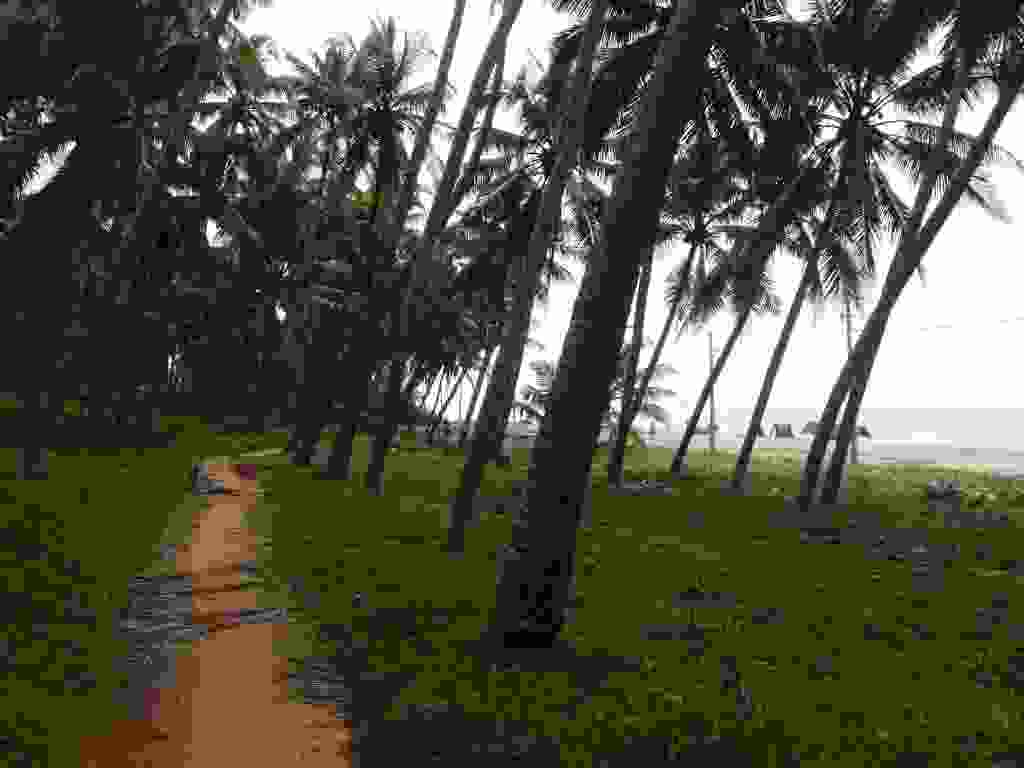
\includegraphics[width=\mywidth]{../wp-content/uploads/2015/11/PB090709-1024x768.jpg} \end{center}

\pagebreak
 Varkala est une célèbre destination touristique pour les occidentaux, beaucoup d'endroits pour faire des massages ayurvédiques ou du yoga. 
\begin{center} 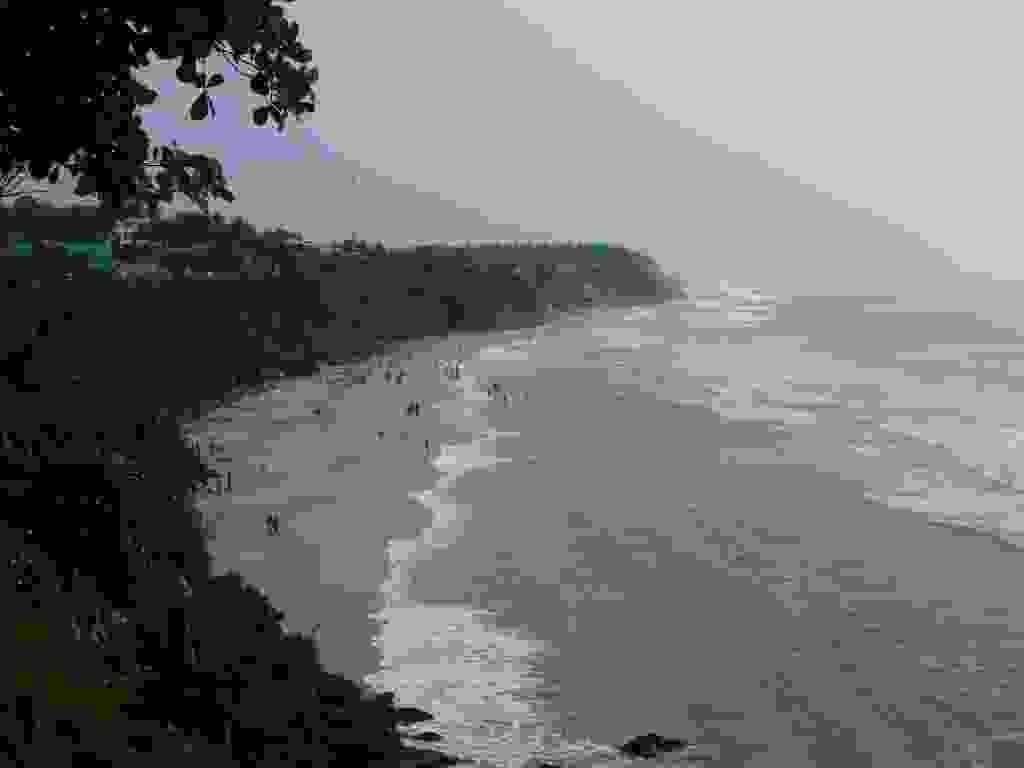
\includegraphics[width=\mywidth]{../wp-content/uploads/2015/11/wpid-oi000373-1024x768.jpg} \end{center}

 Le temple Shree Janardhana Swamy dans le village. 
\begin{center} 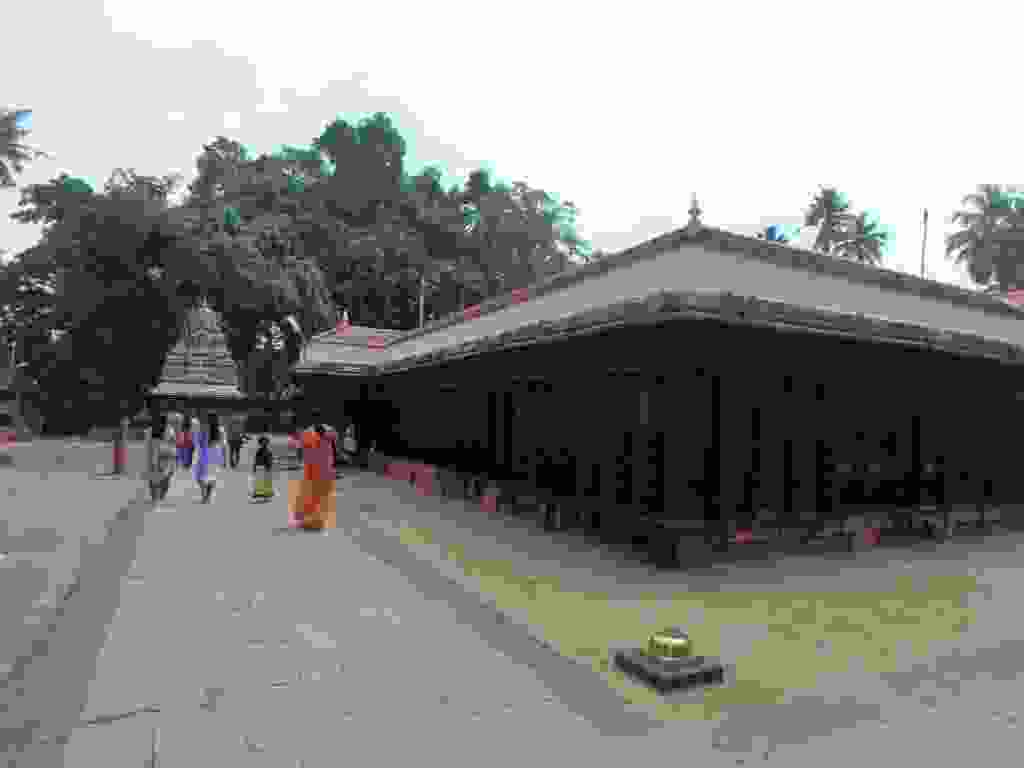
\includegraphics[width=\mywidth]{../wp-content/uploads/2015/11/PB080698-1024x768.jpg} \end{center}
\begin{center} 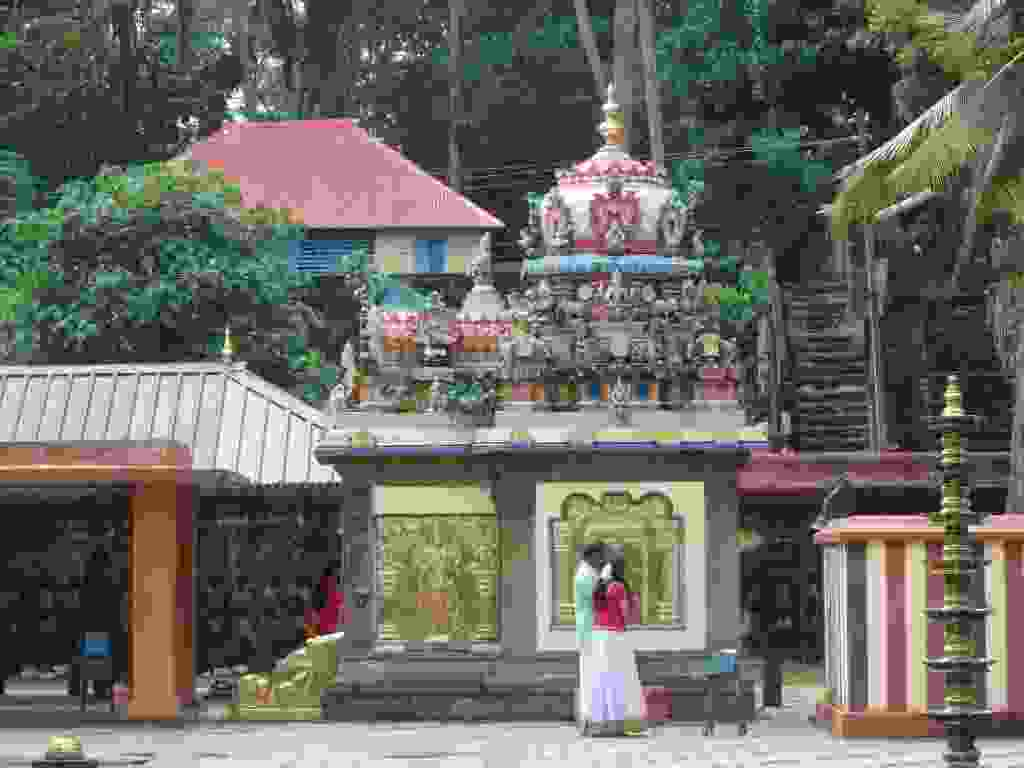
\includegraphics[width=\mywidth]{../wp-content/uploads/2015/11/wpid-oi000379-1024x768.jpg} \end{center}

 Je passe ensuite à Trivandrum la capitale du Kerala. 

 Le temple Sri Padmanabhaswamy, seul les hindous peuvent entrer en respectant la tenue réglementaire. 
\begin{center} 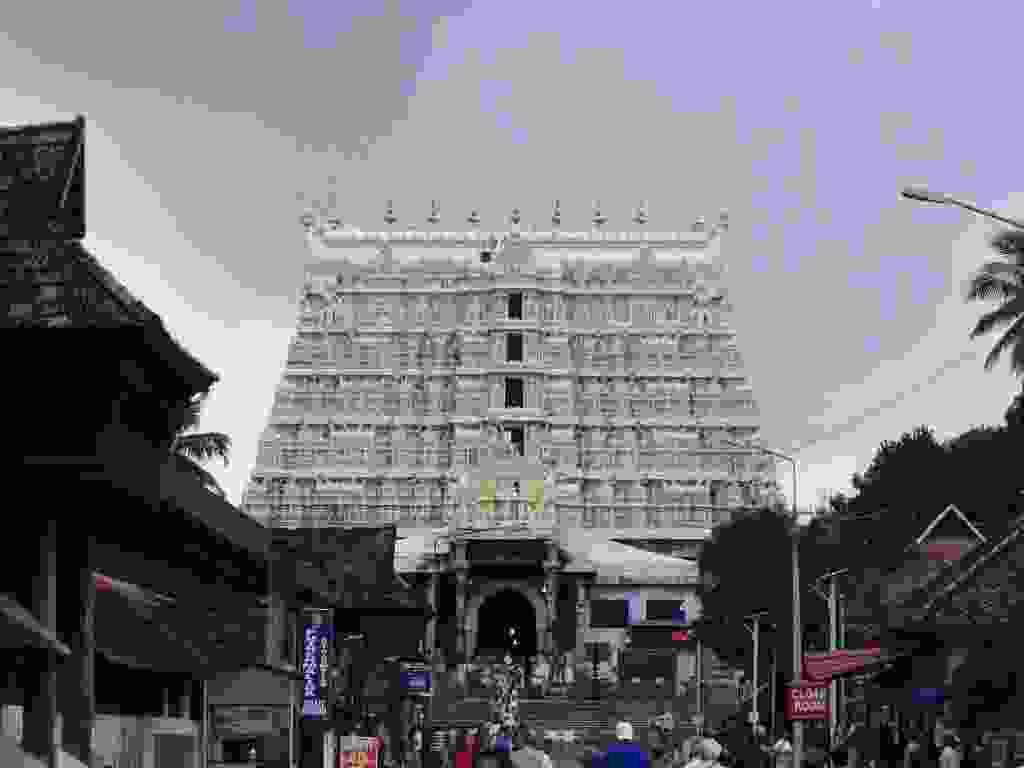
\includegraphics[width=\mywidth]{../wp-content/uploads/2015/11/PB090728-1024x768.jpg} \end{center}
\begin{center} 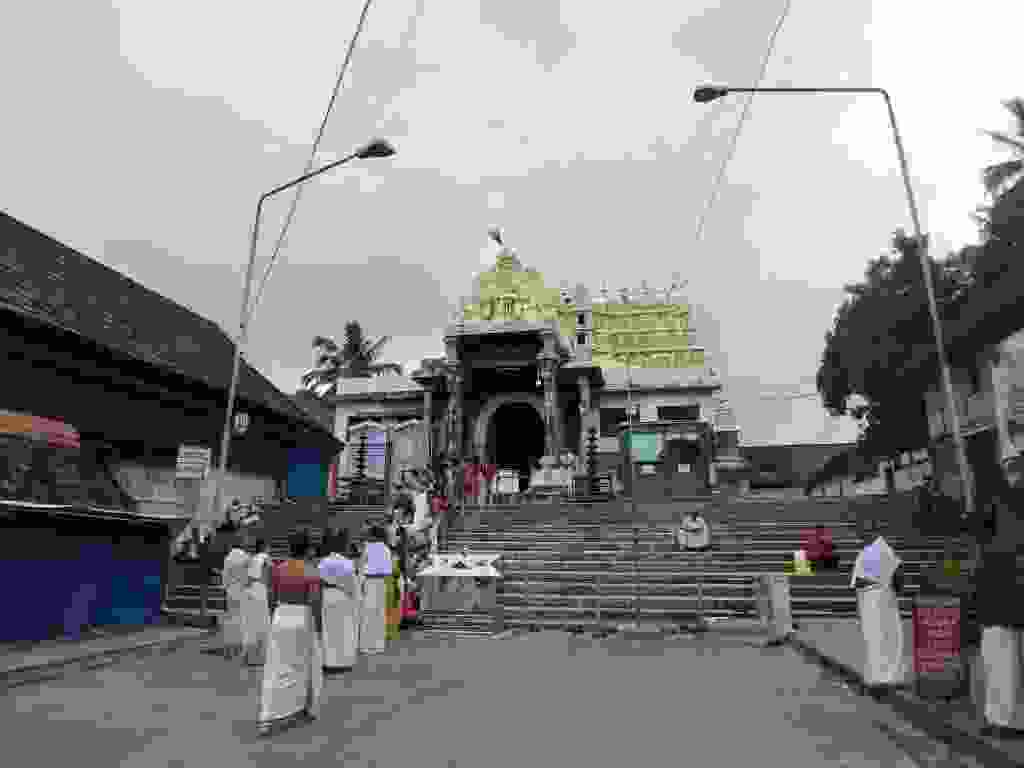
\includegraphics[width=\mywidth]{../wp-content/uploads/2015/11/PB090726-1024x768.jpg} \end{center}

 Musée Napier. 
\begin{center} 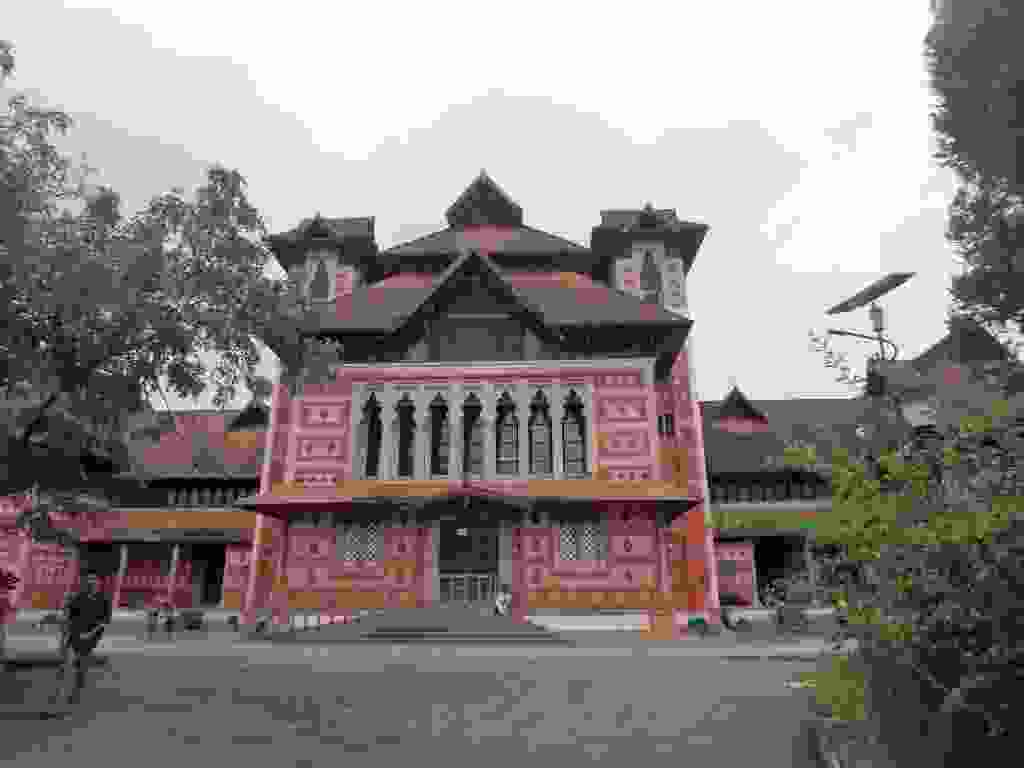
\includegraphics[width=\mywidth]{../wp-content/uploads/2015/11/PB090721-1024x768.jpg} \end{center}

\pagebreak
 Dernière étape dans le Kerala : Kovalam, dans le même esprit que Varkala avec plus de touristes indiens peut-être. 
\begin{center} 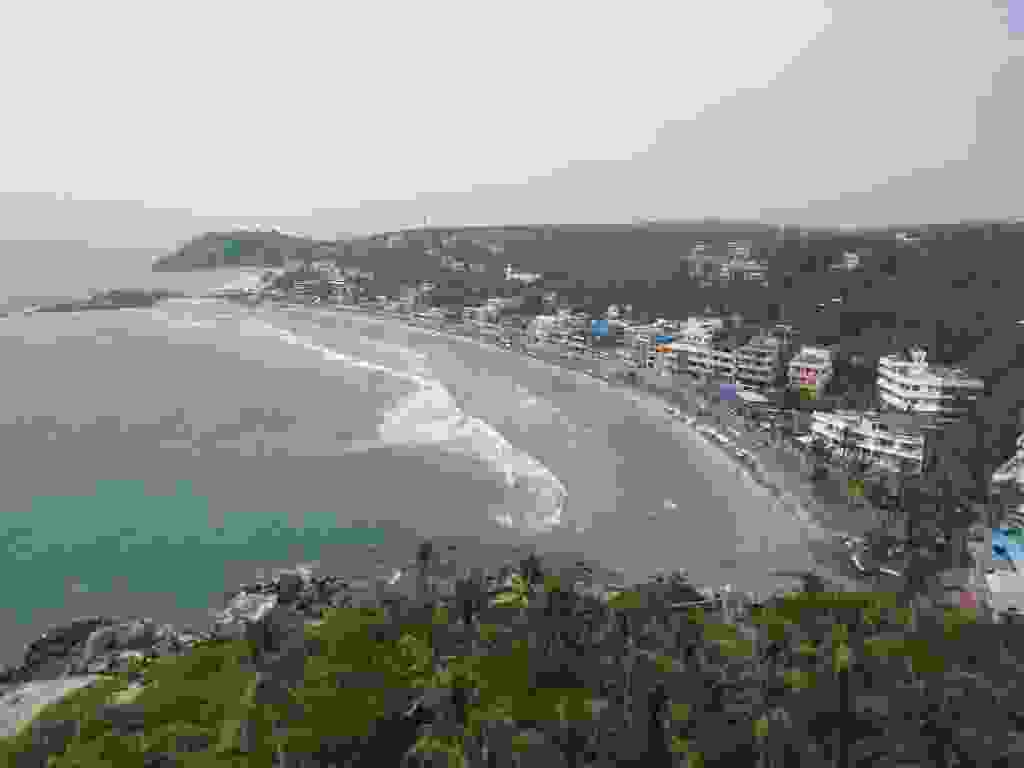
\includegraphics[width=\mywidth]{../wp-content/uploads/2015/11/PB100740-1024x768.jpg} \end{center}
\begin{center} 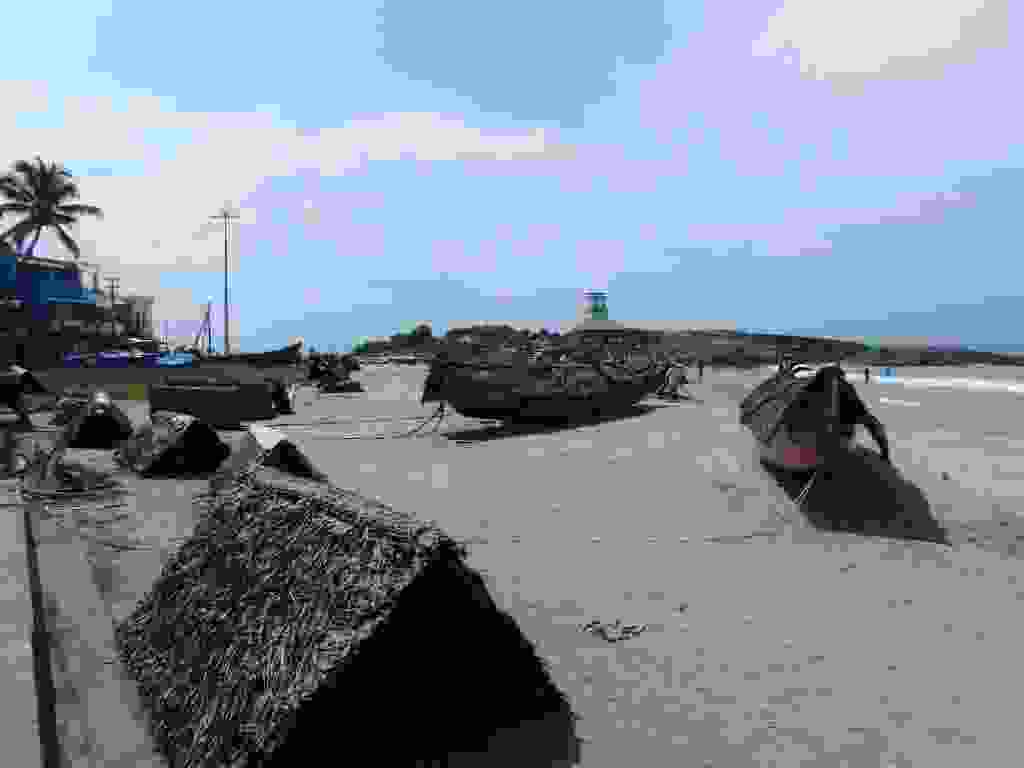
\includegraphics[width=\mywidth]{../wp-content/uploads/2015/11/PB100733-1024x768.jpg} \end{center}
\begin{center} 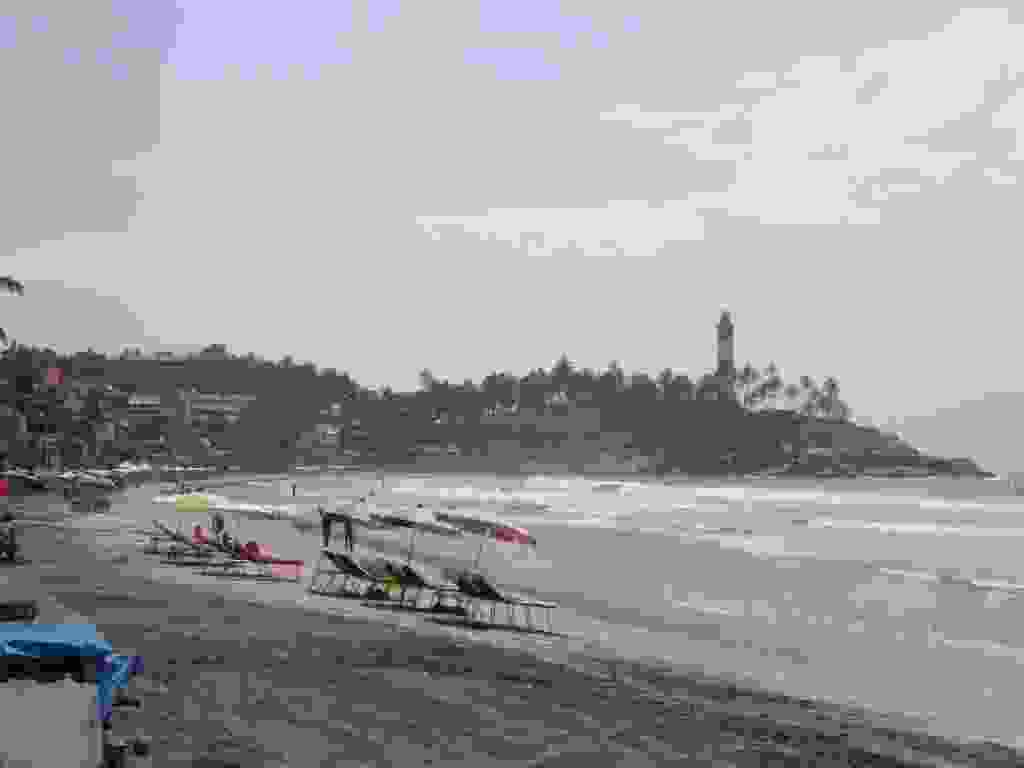
\includegraphics[width=\mywidth]{../wp-content/uploads/2015/11/PB100735-1024x768.jpg} \end{center}
\begin{center} 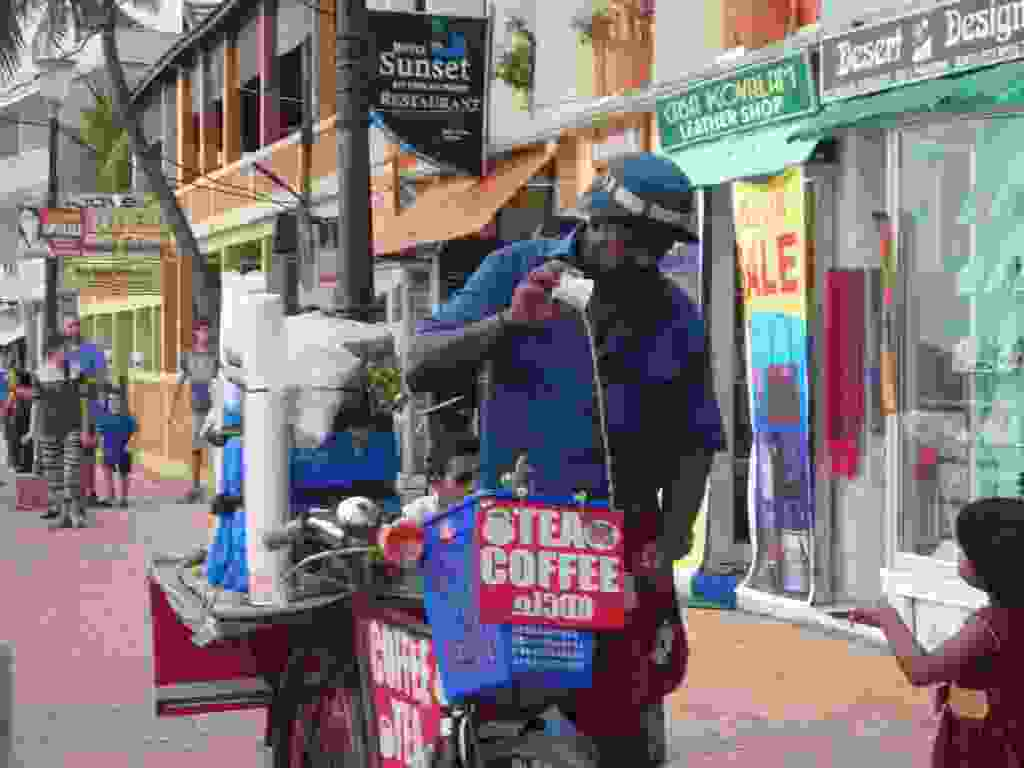
\includegraphics[width=\mywidth]{../wp-content/uploads/2015/11/PB100746-1024x768.jpg} \end{center}

\pagebreak
 En Inde, difficile de trouver de l'alcool hors des lieux touristiques : seulement dans quelques endroits autorisés et à certaines heures. 
\begin{center} 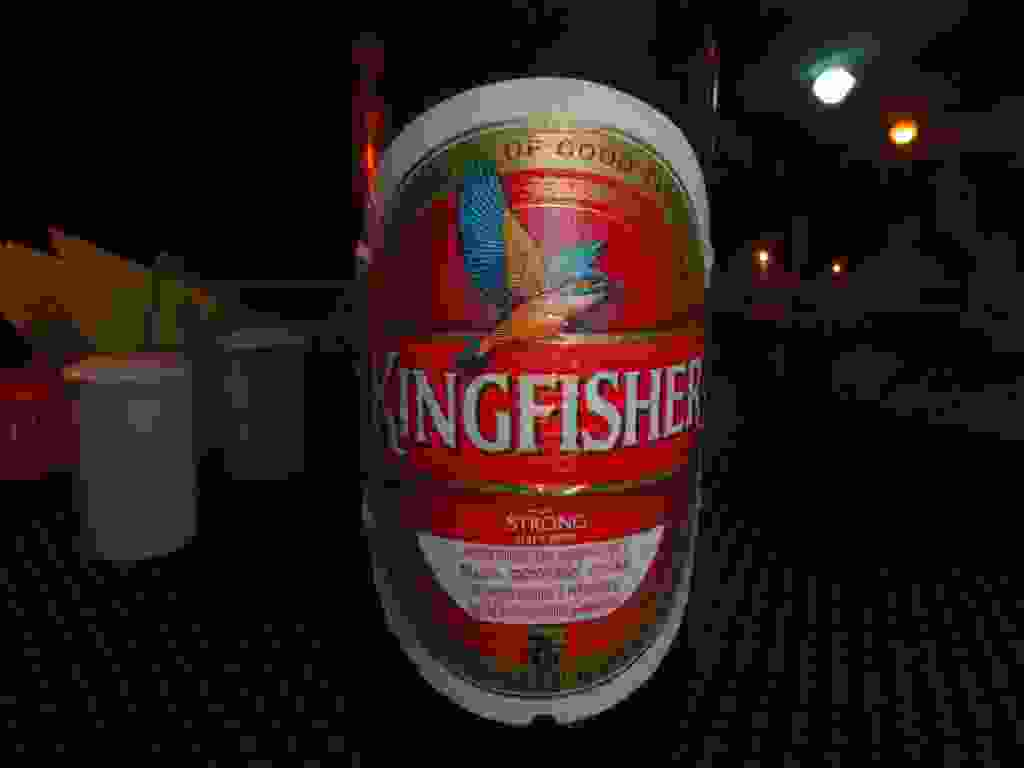
\includegraphics[width=\mywidth]{../wp-content/uploads/2015/11/PB080705-1024x768.jpg} \end{center}

  Côté cuisine, Masala Dosa : crêpe remplie de légumes.
\begin{center} 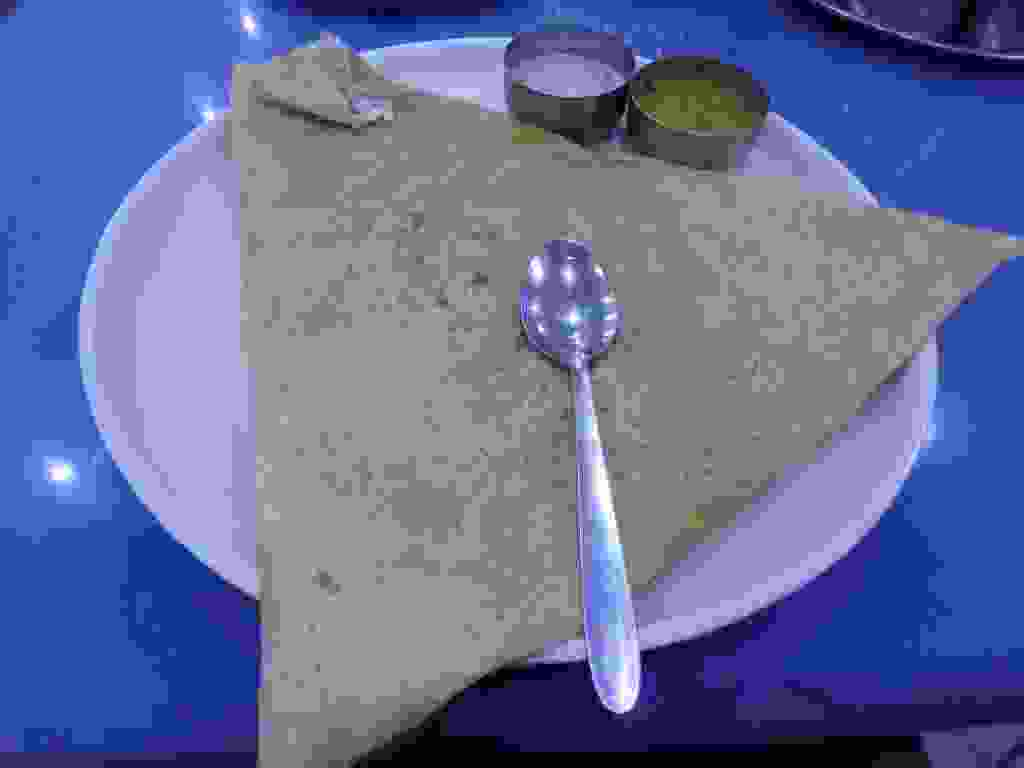
\includegraphics[width=\mywidth]{../wp-content/uploads/2015/11/wpid-oi000363-1024x768.jpg} \end{center}